\documentclass[10pt,conference]{IEEEtran}

\usepackage{amsfonts}
\usepackage[latin1]{inputenc}
\usepackage[english]{babel}
\usepackage{listings}
\usepackage{algorithmic}
\usepackage{float}
%\usepackage[numbers,sort&compress,square]{natbib}
\usepackage{graphicx}
\usepackage{booktabs}
\usepackage{subcaption}
%\usepackage{hyperref}
\usepackage{color}
%\usepackage[usenames,dvipsnames,table]{xcolor}
\usepackage{soul}
\usepackage{xspace}
\usepackage{boxedminipage}
\usepackage{alltt}
\usepackage{multirow}
\usepackage{paralist}
\usepackage{amsmath}
\usepackage{balance}
\definecolor{light-gray}{gray}{0.90}

\floatstyle{ruled}
\newfloat{algorithm}{tbp}{loa}
\floatname{algorithm}{Algorithm}

\newtheorem{definition}{Definition}


 %krams hinter fontadjust ist neu
  \definecolor{lightgrey}{rgb}{0.90,0.90,0.90}
\lstset{escapeinside={(*}{*)}}
  \lstloadlanguages{java}
 \lstdefinelanguage{pseudocode}
  {morekeywords={if, else, initialize, return, for, each, in, global, new}
   }
  \lstset{
    tabsize=2,
    mathescape=true,
    escapeinside={(*}{*)},
    captionpos=t,
    framerule=0pt,
    backgroundcolor=\color{lightgrey},
    basicstyle=\scriptsize\ttfamily,
    keywordstyle=\footnotesize\bfseries,
    numbers=none,
    numberstyle=\tiny,
    numbersep=1pt,
    fontadjust,
    breaklines=true,
    breakatwhitespace=false
  }


% \hypersetup{
% colorlinks=true,
% urlcolor=rltblue,
% linkcolor=rltred,
% citecolor=rltgreen,
% bookmarksnumbered=true,
% pdftitle={EvoSuite at the SBST 2016 Tool Competition},
% pdfauthor={Gordon Fraser and Andrea Arcuri},
% pdfsubject={Test case generation},
% pdfkeywords={Test case generation, unit testing, test
%   oracles, assertions, search based testing}
% }

\definecolor{rltred}{rgb}{0.5,0,0}
\definecolor{rltgreen}{rgb}{0,0.5,0}
\definecolor{rltblue}{rgb}{0,0,0.5}
\definecolor{ScarletRed}{rgb}{0.80,0.00,0.00}



% in draft mode we put \remarks into the margins and do other stuff
% set to \draftfalse for
\newif\ifdraft
%\draftfalse
\drafttrue

\ifdraft
	\marginparwidth=1.3cm
	\marginparsep=5pt
	\newcommand\remark[1]{%
		\mymarginpar{\raggedright\hbadness=10000\tiny\it #1\par}}
	% TODO marker
	\newcommand{\TODO}[1]{\sethlcolor{yellow}\textbf{\textcolor{ScarletRed}{\hl{TODO: #1}}}\xspace}
\else
	\newcommand\remark[1]	{}
	\newcommand{\TODO}[1]{}
\fi

\ifdraft
	\overfullrule3pt
\fi

% We use \FIXME for located problems (``defect'')
\newcommand{\FIXME}[1]{\remark{FIXME: #1}}
\newcommand\parremark[1]	{\par\textbf{REMARK:} #1\par}

\newcommand{\gordon}[1]{\textcolor{blue}{\sf\small\textbf{Gordon:} #1}}
\newcommand{\andrea}[1]{\textcolor{ScarletRed}{\sf\small\textbf{Andrea:} #1}}

% \mathid is used to denote identifiers and slots in formulas
\newcommand{\mathid}[1]{\text{\rmfamily\textit{#1}}}

% But usually, we shall use \|name| instead.
\def\|#1|{\mathid{#1}}

% \codeid is used to denote computer code identifiers
\newcommand{\codeid}[1]{\texttt{#1}}

% But usually, we shall use \<name> instead.
\def\<#1>{\codeid{#1}}

% Our results
\newenvironment{result}%
{\smallskip
\noindent
\let\emph=\textbf
\begin{boxedminipage}{\columnwidth}\begin{center}\em}%
{\end{center}\end{boxedminipage}%
\smallskip
}

\newcommand{\project}[1]{\textsc{#1}\xspace}
\newcommand{\Collections}{\project{Collections}}
\newcommand{\Threeten}{\project{Threeten}}
\newcommand{\Spatial}{\project{Spatial4j}}

\newcommand{\EVOSUITE}{\textsc{EvoSuite}\xspace}
\newcommand{\UtbotConcolic}{\textsc{Utbot-concolic}\xspace}
\newcommand{\TT}{\textsc{T3}\xspace}

\newcommand{\MUTEST}{{\sc $\mu$Test}\xspace}
\newcommand{\CS}{{\sc SF100}\xspace}


\DeclareMathSymbol{,}{\mathpunct}{letters}{"3B}
\DeclareMathSymbol{,}{\mathord}{letters}{"3B}
\DeclareMathSymbol{\decimal}{\mathord}{letters}{"3A}
%%%"

\usepackage{siunitx}
\newcommand{\score}{\num{380.57}\xspace}
\newcommand{\cuts}{\num{65}\xspace}
\newcommand{\budgetShort}{\SI{30}{\second}\xspace}
\newcommand{\budgetLong}{\SI{120}{\second}\xspace}
\newcommand{\avgLinesCoverageRatioShort}{\SI[round-mode=figures,round-precision=3]{51.87307894984616}{\percent}\xspace}
\newcommand{\medLinesCoverageRatioShort}{\SI[round-mode=figures,round-precision=3]{46.666668}{\percent}\xspace}
\newcommand{\avgLinesCoverageRatioLong}{\SI[round-mode=figures,round-precision=3]{62.73892781107692}{\percent}\xspace}
\newcommand{\medLinesCoverageRatioLong}{\SI[round-mode=figures,round-precision=3]{71.71428499999999}{\percent}\xspace}
\newcommand{\avgConditionsCoverageRatioShort}{\SI[round-mode=figures,round-precision=3]{46.11903214169231}{\percent}\xspace}
\newcommand{\medConditionsCoverageRatioShort}{\SI[round-mode=figures,round-precision=3]{47.22222}{\percent}\xspace}
\newcommand{\avgConditionsCoverageRatioLong}{\SI[round-mode=figures,round-precision=3]{56.821364993692306}{\percent}\xspace}
\newcommand{\medConditionsCoverageRatioLong}{\SI[round-mode=figures,round-precision=3]{60.000004}{\percent}\xspace}
\newcommand{\avgMutantsCoverageRatioShort}{\SI[round-mode=figures,round-precision=3]{39.44754914507693}{\percent}\xspace}
\newcommand{\medMutantsCoverageRatioShort}{\SI[round-mode=figures,round-precision=3]{20.353981}{\percent}\xspace}
\newcommand{\avgMutantsCoverageRatioLong}{\SI[round-mode=figures,round-precision=3]{34.111612112}{\percent}\xspace}
\newcommand{\medMutantsCoverageRatioLong}{\SI[round-mode=figures,round-precision=3]{0.0}{\percent}\xspace}
\newcommand{\numTestGenFailedShort}{\num{21}\xspace}
\newcommand{\numTestGenFailedLong}{\num{26}\xspace}


%-------------------------------------------------------------------------
% take the % away on next line to produce the final camera-ready version
\pagestyle{empty}

%-------------------------------------------------------------------------
\begin{document}

%

%\title{Unit Testing Tool competition: Results for EvoSuite}
\title{\EVOSUITE at the SBFT 2023 Tool Competition}


\author{%
  \IEEEauthorblockN{Sebastian Schweikl}
  \IEEEauthorblockA{%
    \textit{University of Passau} \\
    Passau, Germany \\
    sebastian.schweikl@uni-passau.de
  }
  \and
  \IEEEauthorblockN{Gordon Fraser}
  \IEEEauthorblockA{%
    \textit{University of Passau} \\
    Passau, Germany \\
    gordon.fraser@uni-passau.de
  }
  \and
  \IEEEauthorblockN{Andrea Arcuri}
  \IEEEauthorblockA{%
    \textit{Kristiania University College} and\\ \textit{Oslo Metropolitan University} \\
    Oslo, Norway \\
    andrea.arcuri@kristiania.no
  }
}

\maketitle

\begin{abstract}
  \EVOSUITE is an automated unit test generation tool for Java based
  on meta-heuristic search techniques. This paper summarises the
  results and experiences of \EVOSUITE's participation at the 11th
  unit testing competition at SBFT 2023, where \EVOSUITE achieved the
  highest overall score.
\end{abstract}


%-------------------------------------------------------------------------
\section{Introduction}
%
The aim of the annual Java Unit Testing Competition is to evaluate and monitor
the progress on automated test generation. To this end, a new corpus of benchmark
Java classes is created every year, against which various unit test generation tools
are evaluated. This year, the 11th edition of the competition featured a set of \cuts
classes, and five tools. Details about the procedure of the competition, the
technical framework, and the benchmark classes can be found in the competition
report~\cite{SBFT-toolcomp23}. With an overall score of \score, \EVOSUITE achieved the
best result among its competitors.


%-------------------------------------------------------------------------
\section{About EvoSuite}

\EVOSUITE~\cite{FrA11c} is an automatic test generation tool for Java classes.
It takes the name of the target class as input, along with a Java classpath that
locates the class's compiled bytecode and that of its dependencies, and produces
a test suite in JUnit~4 format optimised for code coverage as output.

In a preprocessing phase, \EVOSUITE uses a basic static analysis to collect
information about the relevant classes, such as their constructors, methods
and fields. \EVOSUITE loads these classes into the Java Virtual Machine, and
applies various types of  bytecode instrumentation while doing so. This enables \EVOSUITE
to produce test execution traces, and to avoid test flakiness by replacing
non-deterministic calls with deterministic, mocked versions.

The main execution phase of \EVOSUITE is dedicated to test generation. Here,
meta-heuristic search algorithms are applied to automatically produce JUnit
tests that maximise code coverage. Internally, \EVOSUITE uses a genetic encoding
that represents a test case as variable-length sequence of Java statements
(e.g., primitive statements as well as calls on constructors or methods).
Standard evolutionary search operators (e.g., selection, crossover, mutation)
are adapted for this representation.

\EVOSUITE implements several different evolutionary algorithms that operate on this
representation. Early versions of \EVOSUITE followed the \emph{Whole Test Suite} (WTS)
approach~\cite{GoA_TSE12}, where entire test suites are optimised with
respect to their overall code coverage. A subsequent study~\cite{ea_evaluation}
introduced the \emph{Dynamic Many-Objective Sorting Algorithm} (DynaMOSA)~\cite{dynamosa} algorithm, which was shown
to yield superior results. Unlike WTS, DynaMOSA operates directly at the test case level,
and it is now the default algorithm in \EVOSUITE.

Irrespective of which algorithm is chosen, the search is always driven by fitness
functions. These encode coverage criteria, and \EVOSUITE can optimise for multiple
criteria at the same time. Core fitness functions are based on traditional heuristics
for code coverage, such as branch distance and approach level (see \EVOSUITE's original paper~\cite{GoA_TSE12} for more details.)
Besides this, there are further fitness functions based on mutation
testing~\cite{emse14_mutation} and other basic criteria~\cite{rojas2015combining}.

\EVOSUITE consists of a large code base, of which a large share is
dedicated to avoiding flakiness in the generated tests. This is
achieved using extensive instrumentation and mocking, as well as
post-processing; for example, \EVOSUITE compiles and executes each
test individually to avoid compilation errors (which may be the result
of bugs in \EVOSUITE) or flakiness caused by non-determinism in the
class under test.

Once the available search budget for the main phase has been exhausted,
\EVOSUITE can be configured to run a postprocessing phase where tests are optimised for
readability~\cite{FrA11c,FrA13a}. This includes avoiding test
smells~\cite{panichella2020revisiting}, minimisation to remove redundant tests
and statements, and adding a minimised set of assertions using mutation
analysis~\cite{10.1109/TSE.2011.93}.


%-------------------------------------------------------------------------
\section{Competition Setup}\label{sec:setup}

\EVOSUITE is currently undergoing a significant rewrite to improve the quality
of its internal code base, for example a better use of Java generics to aid
type safety. The latest version (1.2.0) contains the first fruits of this effort,
but also introduced regressions that still existed at the time the competition was
hold. For this reason, the same version (1.1.0) as in previous years was used.
The remaining setup was largely similar to the 2022 iteration: DynaMOSA~\cite{dynamosa}
was chosen as search algorithm, and \EVOSUITE was configured with the parameters
established in prior years, which mainly uses the tuned default
values~\cite{arcuri2013parameter} and default coverage criteria~\cite{rojas2015combining}.
%
% No new features were added in this version, but support
% for Java 9+ was added, several bugs were fixed, and a major refactoring was applied
% to improve the code quality with respect to the
% use of Java Generics internally. While several smaller bugfixes were applied in
% the run-up to the 2021 competition, no further optimisation or testing was
% applied for 2022.
%
While in previous years the competition only rewarded code coverage, this year
test case readability was also factored in. To account for this, the new configuration
enables a test minimisation step, and filters regression assertions using mutation analysis.
%
The time budget was again distributed by allocating \SI{50}{\percent} of the overall time
set by the competition organisers for the search, and the other \SI{50}{\percent} equally to
the remaining phases (e.g., assertion generation, compile-check, flakiness-check).



%-------------------------------------------------------------------------
\section{Results}

%\begin{figure}
%  \centering
%  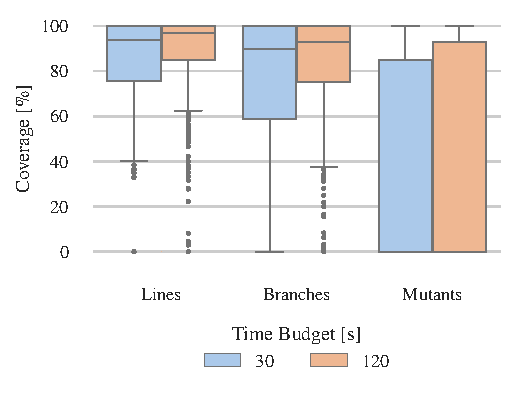
\includegraphics[width=\columnwidth]{data/CoverageBoxV}
%  \caption{Coverage results achieved in the competition.}
%  \label{fig:results}
%\end{figure}

\begin{figure}
  \centering

  \begin{subfigure}{\columnwidth}
    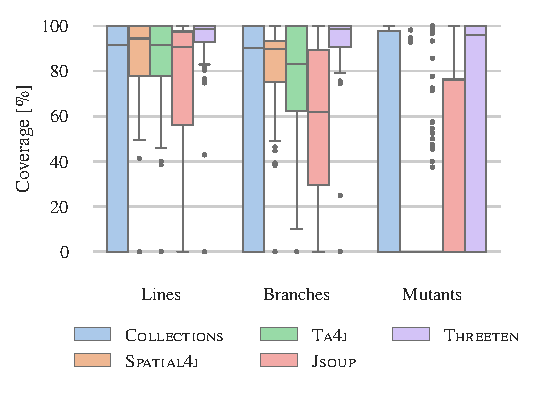
\includegraphics[width=\linewidth]{data/CoverageByBenchmark30.pdf}
    \caption{Results achieved in the competition with a budget of \budgetShort}
    \label{fig:results30}
  \end{subfigure}

  \begin{subfigure}{\columnwidth}
    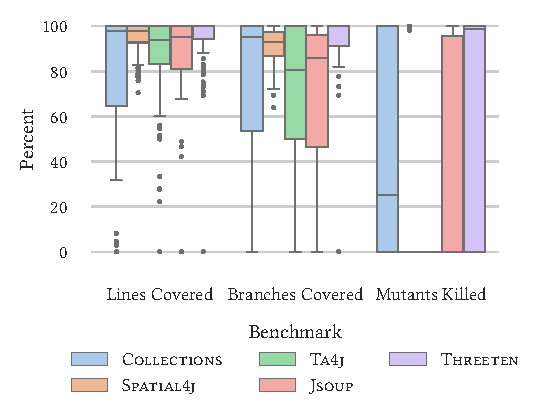
\includegraphics[width=\linewidth]{data/CoverageByBenchmark120.pdf}
    \caption{Results achieved in the competition with a budget of \budgetLong}
    \label{fig:results120}
  \end{subfigure}

  \caption{Coverage results achieved by \EVOSUITE per each of the 5~projects
    used in the competition}
  \label{fig:figures}
\end{figure}


With an overall score of \score, \EVOSUITE was the highest ranking tool
(rank \rank) in the competition. The score is computed as the weighted
sum between the rankings for coverage (rank \rankCoverage) and understandability
(rank \rankUnderstandability). We refer to the competition report~\cite{SBFT-toolcomp23}
for more details.

The coverage \EVOSUITE achieved on the \cuts classes distributed across the \projects
projects used in the competition is illustrated in Figure~\ref{fig:results30} for a search
budget of \budgetShort, and in Figure~\ref{fig:results120} for a budget of \budgetLong.
The average line and branch coverage for the \budgetShort budget is
\avgLinesCoverageRatioShort and \avgConditionsCoverageRatioShort, and
increases to \avgLinesCoverageRatioLong and \avgConditionsCoverageRatioLong
for the \budgetLong budget. The average mutation coverage is \avgMutantsCoverageRatioShort
and \avgMutantsCoverageRatioLong, respectively.

As stated in the competition report~\cite{SBFT-toolcomp23} \EVOSUITE is the
only tool for which the median number of generated tests \emph{decreases}
from \num{35} for the \budgetShort budget to \num{23.5} for the \budgetLong budget.
As stated before, \EVOSUITE tries to apply additional post-processing steps to remove
redundant tests. However, in case of the \budgetShort budget most time is spent on test
generation and only little time remains for minimisation.

% While the results for line coverage and branch coverage are similar, the
% mutation scores are substantially lower. The mutation scores on the \Threeten
% classes are highest compared to the other projects from which classes were taken.

% https://github.com/JUnitContest/JUGE/blob/master/benchmarktool/src/main/java/sbst/benchmark/Main.java#L160
In \numTestGenFailedShort cases \EVOSUITE failed to generate any tests with a
budget of \budgetShort. However, this might have been caused by problems in the
infrastructure\footnote{https://github.com/JUnitContest/JUGE/}
of the competition as we found no crashes or error messages
of \EVOSUITE itself. Instead, the log files contained the error message
``Error: null'' triggered by line~160 in the \texttt{main()} method of
the \texttt{sbst.benchmark.Main} class. Here, \EVOSUITE is invoked with an
\texttt{IBenchmarkTask} object as input which seems to have not been properly
initialised.
%
The same error also ocurred in 13 of \numTestGenFailedLong
cases with a budget of \budgetLong. In the remaining 4 cases, \EVOSUITE crashed
with an \texttt{OutOfMemoryError}. % while generating or postprocessing tests.

% threeten-extra-99 (2×)
% Test generation aborted
% Out of Memory Error GH overhead limit exceeded

% collections-10
% Crash
% java.lang.OutOfMemoryError: Java heap space during test suite minimisation

% ta4j-79
% java.lang.OutOfMemoryError: GC overhead limit exceeded while post-processing tests

\begin{figure}
  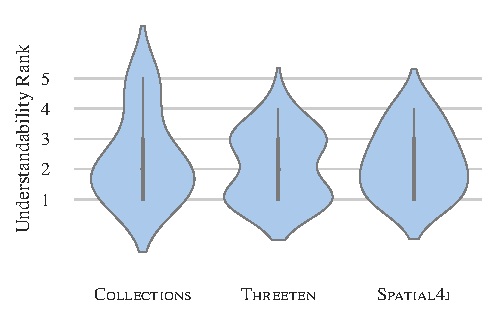
\includegraphics[width=\columnwidth]{./data/understandability}
  \caption{Distribution of test case understandability, ranked from 1 (best) to 5 (worst), per project}
  \label{fig:readability}
\end{figure}

For the first time, the competition included a human study with 13
participants to assess test case readability. For each of the projects \Collections,
\Threeten, and \Spatial, participants were presented a test case
generated by each of the six competing tools, covering the same method under
test. The participants were then asked to rank the tests per project
on a scale from 1 (best) to 5 (worst), in terms of readability. Overall,
\EVOSUITE achieved the 2nd best rating (rank 2.23 on average),
preceded by \UtbotConcolic (2.13 on average). \EVOSUITE's rank distribution
is shown in Figure~\ref{fig:readability}.

Most participants found \EVOSUITE-generated tests to be readable. When
\EVOSUITE ranked best, they positively highlighted the thoroughness of
generated assertions, using edge cases as inputs, and the fact that
tests where short. When \EVOSUITE ranked worst, participants
criticised the lack of comments and descriptive test names,
repetitiveness in the code, and needless assertions. While \EVOSUITE's
competition setup enabled test and assertion minimisation, this is a
computationally very expensive process, and it is likely \EVOSUITE was
sometimes unable to finish in time, leaving tests unoptimised. In
particilar, there are two aspects of this minimisation: The first
minimisation phase attempts to remove all statements in a test that
are irrelevant for achieving the test's coverage goals; the second
minimisation phase consists of selecting a minimal subset of test
assertions that are sufficient to detect all code mutants the test is
capable of detecting. If either of these phases exceeds the allocated
time budget it is cancelled, and \EVOSUITE returns the non-minimised
tests.

Among the tests for \Collections the longest one was produced by
\EVOSUITE.  Interestingly, it ranked both highest and lowest, with one
participant stating it was ``the most complete'', while another
suggested the code being longer makes it ``more confusing''. As a
general trend, participants seemed to prefer shorter, more cohesive
tests with assertions that only check one particular aspect of the
method under test.

%-------------------------------------------------------------------------
\section{Conclusions}


This paper describes the results and experiences of \EVOSUITE's
participation in the 11th SBST Java Unit Testing Tool Contest. On
average, \EVOSUITE achieved \avgConditionsCoverageRatioLong branch
coverage, \avgLinesCoverageRatioLong line coverage, and a mutation
score of \avgMutantsCoverageRatioLong, using a search budget of
\budgetLong on the \cuts classes considered for the
competition. Overall, this results in a score of \score, which is the
highest score of all competing tools.


To learn more about \EVOSUITE, visit our Web site:
\begin{center}
%\url{http://evosuite.org/}
\texttt{http://www.evosuite.org}
\end{center}


%-------------------------------------------------------------------------

%\noindent
\textbf{Acknowledgments:} Many thanks to all the contributors to
\EVOSUITE.
%This project has been supported by EPSRC project % ``GREATEST''
%EP/N023978/2.


%-------------------------------------------------------------------------
%\def\IEEEbibitemsep{5pt plus 1pt}
%\def\IEEEbibitemsep{6pt}
%\clearpage
\balance
\bibliographystyle{IEEEtranS}
\bibliography{papers}

\end{document}


%%% Local Variables:
%%% mode: latex
%%% TeX-master: t
%%% End:
